This appendix contains all the graphs and the tables related to the write experiments conducted, and of the comparison with the related work. Results are reported first expressed as latency (measured in seconds) and then as throughput (measured in rows/seconds). Latency was directly measured, while throughput was computed from the latency and table size.


%%%%%%%%%%%%%%%%%%%%%%%%%%%%%%%%%%%%%%%%%%%%%%%%%%%%%%%%%%%%%%%%%
%%%%%%%%%%%%              LATENCY             %%%%%%%%%%%%%%%%%%%
%%%%%%%%%%%%%%%%%%%%%%%%%%%%%%%%%%%%%%%%%%%%%%%%%%%%%%%%%%%%%%%%%
\begin{figure}
    \centering
    \begin{minipage}[b]{\textwidth}
        \centering
        \captionof{table}[Write experiment - Latency - 1 CPU core]{Write experiment results expressed as latency. The experiment was performed with one \glstext{CPU} core.}
        \label{tbl:appx_res_write_time_1_core_HID}
        \begin{tabular}{c r S[table-format=5.5] S[table-format=5.5] S[table-format=5.5]} 
            \toprule
            \multirow{2}{*}{{Pipeline\Tstrut\Bstrut}} & \multirow{2}{*}{{\thead{Number\\ of rows}}} & {\multirow{2}{*}{{\thead{Latency \\ (seconds)}}}} & \multicolumn{2}{c}{{\thead{Latency (seconds) \\95\% Confidence Interval}}}\\
                                                      &                                             &                                                   & {low} & {high}\\
            \midrule
            \multirow{5}{4em}{Hudi\\Legacy} & 10K  &    50.72779 &   50.11508 &   51.31597\\
                                            & 100K &    59.77647 &   59.10732 &   60.48278\\
                                            & 1M   &   108.56462 &  108.01696 &  109.06968\\
                                            & 6M   &   473.38310 &  472.30635 &  474.45390\\
                                            & 60M  &  2341.08359 & 2334.15850 & 2347.68142\\
            \midrule
            \multirow{5}{4em}{Iceberg\\PyIceberg} & 10K  &     1.19507 &    1.13429 &    1.26015\\
                                                  & 100K &     1.19962 &    1.14105 &    1.25251\\
                                                  & 1M   &     1.72148 &    1.69402 &    1.74827\\
                                                  & 6M   &     3.56635 &    3.50274 &    3.64406\\
                                                  & 60M  &    23.50784 &   23.46474 &   23.54621\\
            \midrule
            \multirow{5}{4em}{Delta Lake\\delta-rs} & 10K  &     1.26280 &    1.25128 &    1.27656\\
                                                    & 100K &     1.30721 &    1.27933 &    1.32999\\
                                                    & 1M   &     8.52018 &    8.34308 &    8.70174\\
                                                    & 6M   &    16.30152 &   15.92007 &   16.66990\\
                                                    & 60M  &   134.15567 &  131.76812 &  136.58794\\
            \bottomrule
        \end{tabular}
    \end{minipage}
    \begin{minipage}[b]{\textwidth}
        \centering
        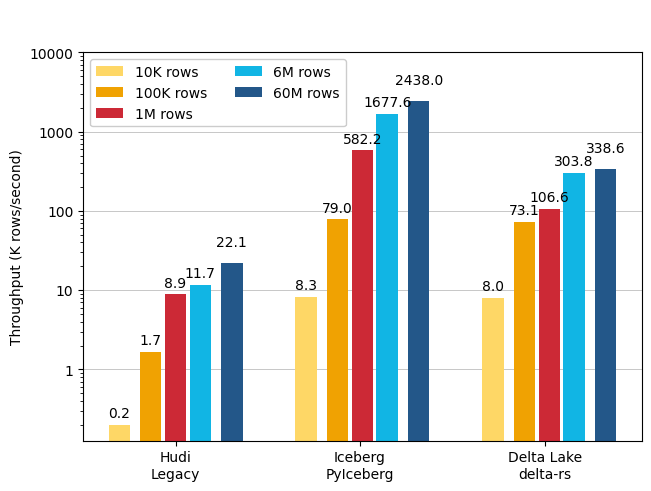
\includegraphics[width=\textwidth]{figures/7-appendix/results_diagrams/write/hudi_iceberg_delta/write_throughput_1_core.png}
        \caption[Histogram of the write experiment - Latency - 1 CPU core]{Histogram in log-scale of the write experiment results expressed as latency. The experiment was performed with one \glstext{CPU} core.}
        \label{fig:appx_res_write_time_1_core_HID}
    \end{minipage}
\end{figure}


\begin{figure}
    \centering
    \begin{minipage}[b]{\textwidth}
        \centering
        \captionof{table}[Write experiment - Latency - 2 CPU cores]{Write experiment results expressed as latency. The experiment was performed with two \glstext{CPU} cores.}
        \label{tbl:appx_res_write_time_2_cores_HID}
        \begin{tabular}{c r S[table-format=5.5] S[table-format=5.5] S[table-format=5.5]} 
            \toprule
            \multirow{2}{*}{{Pipeline\Tstrut\Bstrut}} & \multirow{2}{*}{{\thead{Number\\ of rows}}} & {\multirow{2}{*}{{\thead{Latency \\ (seconds)}}}} & \multicolumn{2}{c}{{\thead{Latency (seconds) \\95\% Confidence Interval}}}\\
                                                      &                                             &                                                   & {low} & {high}\\
            \midrule
            \multirow{5}{4em}{Hudi\\Legacy} & 10K  &    50.72779 &   50.11508 &   51.31597\\
                                            & 100K &    59.77647 &   59.10732 &   60.48278\\
                                            & 1M   &   108.56462 &  108.01696 &  109.06968\\
                                            & 6M   &   473.38310 &  472.30635 &  474.45390\\
                                            & 60M  &  2341.08359 & 2334.15850 & 2347.68142\\
            \midrule
            \multirow{5}{4em}{Iceberg\\PyIceberg} & 10K  &     1.19507 &    1.13429 &    1.26015\\
                                                  & 100K &     1.19962 &    1.14105 &    1.25251\\
                                                  & 1M   &     1.72148 &    1.69402 &    1.74827\\
                                                  & 6M   &     3.56635 &    3.50274 &    3.64406\\
                                                  & 60M  &    23.50784 &   23.46474 &   23.54621\\
            \midrule
            \multirow{5}{4em}{Delta Lake\\delta-rs} & 10K  &     1.26280 &    1.25128 &    1.27656\\
                                                    & 100K &     1.30721 &    1.27933 &    1.32999\\
                                                    & 1M   &     8.52018 &    8.34308 &    8.70174\\
                                                    & 6M   &    16.30152 &   15.92007 &   16.66990\\
                                                    & 60M  &   134.15567 &  131.76812 &  136.58794\\
            \bottomrule
        \end{tabular}
    \end{minipage}
    \begin{minipage}[b]{\textwidth}
        \centering
        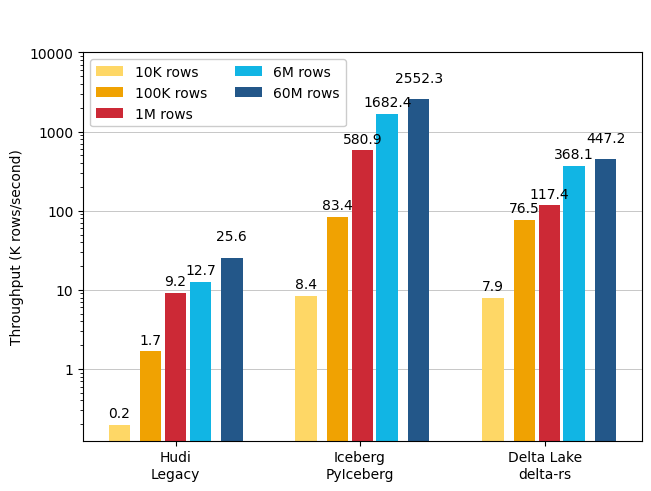
\includegraphics[width=\textwidth]{figures/7-appendix/results_diagrams/write/hudi_iceberg_delta/write_throughput_2_core.png}
        \caption[Histogram of the write experiment - Latency - 2 CPU cores]{Histogram in log-scale of the write experiment results expressed as latency. The experiment was performed with two \glstext{CPU} cores.}
        \label{fig:appx_res_write_time_2_cores_HI}
    \end{minipage}
\end{figure}

\begin{figure}
    \centering
    \begin{minipage}[b]{\textwidth}
        \centering
        \captionof{table}[Write experiment - Latency - 4 CPU cores]{Write experiment results expressed as latency. The experiment was performed with four \glstext{CPU} cores.}
        \label{tbl:appx_res_write_time_4_cores_HDI}
        \begin{tabular}{c r S[table-format=5.5] S[table-format=5.5] S[table-format=5.5]} 
            \toprule
            \multirow{2}{*}{{Pipeline\Tstrut\Bstrut}} & \multirow{2}{*}{{\thead{Number\\ of rows}}} & {\multirow{2}{*}{{\thead{Latency \\ (seconds)}}}} & \multicolumn{2}{c}{{\thead{Latency (seconds) \\95\% Confidence Interval}}}\\
                                                      &                                             &                                                   & {low} & {high}\\
            \midrule
            \multirow{5}{4em}{Hudi\\Legacy} & 10K  &    51.27146 &   50.60985 &   51.91787\\
                                            & 100K &    59.51401 &   58.85512 &   60.13737\\
                                            & 1M   &   108.80723 &  108.29144 &  109.36979\\
                                            & 6M   &   481.95870 &  480.98472 &  482.90019\\
                                            & 60M  &  2346.10873 & 2337.17580 & 2355.21233\\
            \midrule
            \multirow{5}{4em}{Iceberg\\PyIceberg} & 10K  &     1.19528 &    1.16100 &    1.22659\\
                                                  & 100K &     1.25475 &    1.21873 &    1.28507\\
                                                  & 1M   &     1.63161 &    1.58639 &    1.67295\\
                                                  & 6M   &     3.54488 &    3.51441 &    3.57131\\
                                                  & 60M  &    24.00535 &   23.89706 &   24.15370\\
            \midrule
            \multirow{5}{4em}{Delta Lake\\delta-rs} & 10K  &     1.21684 &    1.20238 &    1.23306\\
                                                    & 100K &     1.33653 &    1.32313 &    1.35043\\
                                                    & 1M   &     8.41863 &    8.24595 &    8.60309\\
                                                    & 6M   &    16.22345 &   15.83116 &   16.58556\\
                                                    & 60M  &   124.06139 &  121.16237 &  126.54771\\
            \bottomrule
        \end{tabular}
    \end{minipage}
    \begin{minipage}[b]{\textwidth}
        \centering
        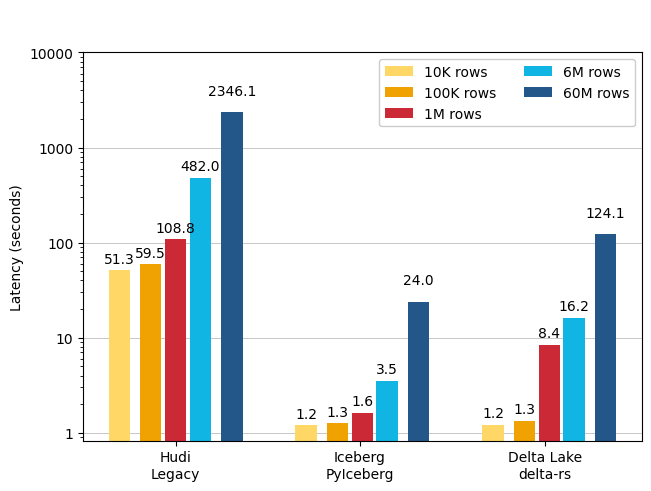
\includegraphics[width=\textwidth]{figures/7-appendix/results_diagrams/write/hudi_iceberg_delta/write_time_4_core.png}
        \caption[Histogram of the write experiment - Latency - 4 CPU cores]{Histogram in log-scale of the write experiment results expressed as latency. The experiment was performed with four \glstext{CPU} cores.}
        \label{fig:appx_res_write_time_4_cores_HID}
    \end{minipage}
\end{figure}

\begin{figure}
    \centering
    \begin{minipage}[b]{\textwidth}
        \centering
        \captionof{table}[Write experiment - Latency - 8 CPU cores]{Write experiment results expressed as latency. The experiment was performed with eight \glstext{CPU} cores.}
        \label{tbl:appx_res_write_time_8_cores_HID}
        \begin{tabular}{c r S[table-format=5.5] S[table-format=5.5] S[table-format=5.5]} 
            \toprule
            \multirow{2}{*}{{Pipeline\Tstrut\Bstrut}} & \multirow{2}{*}{{\thead{Number\\ of rows}}} & {\multirow{2}{*}{{\thead{Latency \\ (seconds)}}}} & \multicolumn{2}{c}{{\thead{Latency (seconds) \\95\% Confidence Interval}}}\\
                                                      &                                             &                                                   & {low} & {high}\\
            \midrule
            \multirow{5}{4em}{Hudi\\Legacy} & 10K  &    51.22598 &   50.58730 &   51.82630\\
                                            & 100K &    60.28808 &   59.77863 &   60.76677\\
                                            & 1M   &   109.38179 &  108.91121 &  109.85272\\
                                            & 6M   &   475.97284 &  474.80788 &  477.12164\\
                                            & 60M  &  2324.80740 & 2319.16036 & 2331.08460\\
            \midrule
            \multirow{5}{4em}{Iceberg\\PyIceberg} & 10K  &     1.21822 &    1.15914 &    1.29076\\
                                                  & 100K &     1.24858 &    1.21985 &    1.27629\\
                                                  & 1M   &     1.71908 &    1.70410 &    1.73150\\
                                                  & 6M   &     3.53248 &    3.47337 &    3.60968\\
                                                  & 60M  &    23.62313 &   23.56093 &   23.70051\\
            \midrule
            \multirow{5}{4em}{Delta Lake\\delta-rs} & 10K  &     1.35965 &    1.24849 &    1.57041\\
                                                    & 100K &     1.29220 &    1.26557 &    1.31120\\
                                                    & 1M   &     8.29498 &    8.14343 &    8.46028\\
                                                    & 6M   &    15.72410 &   15.23956 &   16.17634\\
                                                    & 60M  &   121.89214 &  119.51899 &  124.13425\\
            \bottomrule
        \end{tabular}
    \end{minipage}
    \begin{minipage}[b]{\textwidth}
        \centering
        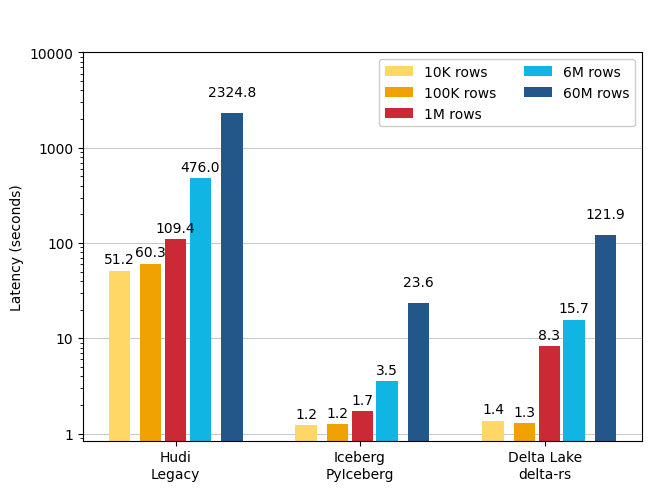
\includegraphics[width=\textwidth]{figures/7-appendix/results_diagrams/write/hudi_iceberg_delta/write_time_8_core.png}
        \caption[Histogram of the write experiment - Latency - 8 CPU cores]{Histogram in log-scale of the write experiment results expressed as latency. The experiment was performed with eight \glstext{CPU} cores.}
        \label{fig:appx_res_write_time_8_cores_HID}
    \end{minipage}
\end{figure}



%%%%%%%%%%%%%%%%%%%%%%%%%%%%%%%%%%%%%%%%%%%%%%%%%%%%%%%%%%%%%%%%%
%%%%%%%%%%%%             THROUGHPUT           %%%%%%%%%%%%%%%%%%%
%%%%%%%%%%%%%%%%%%%%%%%%%%%%%%%%%%%%%%%%%%%%%%%%%%%%%%%%%%%%%%%%%

\begin{figure}
    \centering
    \begin{minipage}[b]{\textwidth}
        \centering
        \captionof{table}[Write experiment - Throughput - 1 CPU core]{Write experiment results expressed as throughput. The experiment was performed with one \glstext{CPU} core.}
        \label{tbl:appx_res_write_throughput_1_core_HID}
        \begin{tabular}{c r S[table-format=7.5] S[table-format=7.5] S[table-format=7.5]} 
            \toprule
            \multirow{2}{*}{{Pipeline\Tstrut\Bstrut}} & \multirow{2}{*}{{\thead{Number\\ of rows}}} & {\multirow{2}{*}{{\thead{Throughput \\ (k rows/second)}}}} & \multicolumn{2}{c}{{\thead{Throughput (k rows/second) \\95\% Confidence Interval}}}\\
                                                      &                                             &                                                          & {low} & {high}\\
            \midrule
            \multirow{5}{4em}{Hudi\\Legacy} & 10K  &   199.05274 &   196.23277 &   202.02946\\
                                            & 100K &  1679.09052 &  1661.20316 &  1697.45005\\
                                            & 1M   &  8914.42526 &  8852.55259 &  8976.77534\\
                                            & 6M   & 11722.20533 & 11698.43772 & 11749.66636\\
                                            & 60M  & 22089.60777 & 21959.12848 & 22215.58201\\
            \midrule
            \multirow{5}{4em}{Iceberg\\PyIceberg} & 10K  &    8305.21414 &    8097.47741 &    8552.13678\\
                                                  & 100K &   79036.57962 &   76974.09347 &   81866.64251\\
                                                  & 1M   &  582172.95332 &  557726.35662 &  601411.81000\\
                                                  & 6M   & 1677621.61097 & 1660186.12626 & 1697038.45776\\
                                                  & 60M  & 2438044.51673 & 2420738.20916 & 2453683.12353\\
            \midrule
            \multirow{5}{4em}{Delta Lake\\delta-rs} & 10K  &   7994.34761 &   7909.77029 &   8076.10878\\
                                                    & 100K &  73099.23983 &  71965.37802 &  74753.62951\\
                                                    & 1M   & 106583.58073 & 104803.16761 & 108218.77550\\
                                                    & 6M   & 303774.53053 & 298336.72214 & 309493.32990\\
                                                    & 60M  & 338610.80463 & 333246.70441 & 343674.23184\\
                                                      
            \bottomrule
        \end{tabular}
    \end{minipage}
    \begin{minipage}[b]{\textwidth}
        \centering
        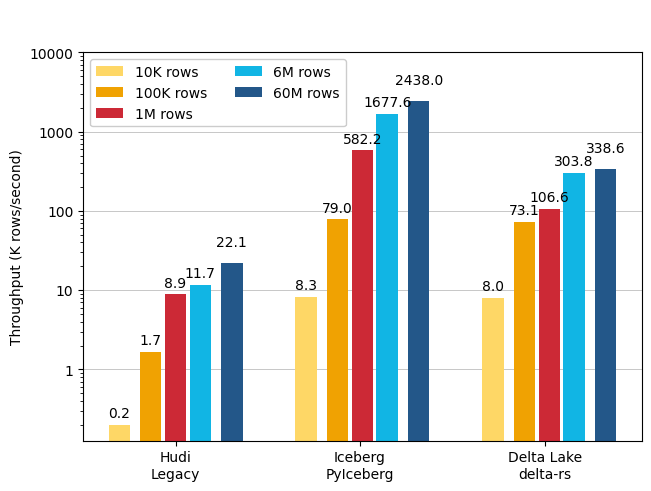
\includegraphics[width=\textwidth]{figures/7-appendix/results_diagrams/write/hudi_iceberg_delta/write_throughput_1_core.png}
        \caption[Histogram of the write experiment - Throughput - 1 CPU core]{Histogram in log-scale of the write experiment results expressed as throughput. The experiment was performed with one \glstext{CPU} core.}
        \label{fig:appx_res_write_throughput_1_core_HID}
    \end{minipage}
\end{figure}

\begin{figure}
    \centering
    \begin{minipage}[b]{\textwidth}
        \centering
        \captionof{table}[Write experiment - Throughput - 2 CPU cores]{Write experiment results expressed as throughput. The experiment was performed with two \glstext{CPU} cores.}
        \label{tbl:appx_res_write_throughput_2_cores_HID}
        \begin{tabular}{c r S[table-format=7.5] S[table-format=7.5] S[table-format=7.5]}  
            \toprule
            \multirow{2}{*}{{Pipeline\Tstrut\Bstrut}} & \multirow{2}{*}{{\thead{Number\\ of rows}}} & {\multirow{2}{*}{{\thead{Throughput \\ (k rows/second)}}}} & \multicolumn{2}{c}{{\thead{Throughput (k rows/second) \\95\% Confidence Interval}}}\\
                                                      &                                             &                                                          & {low} & {high}\\
            \midrule
            \multirow{5}{4em}{Hudi\\Legacy}      & 10K  &   197.13059  &   194.87110  &   199.54075\\
                                                & 100K &  1672.89911  &  1653.36326  &  1691.83772\\
                                                & 1M   &  9211.10364  &  9168.45112  &  9257.80572\\
                                                & 6M   & 12674.72383  & 12646.11798  & 12703.61911\\
                                                & 60M  & 25629.15745  & 25557.13028  & 25705.19531\\
            \midrule
            \multirow{5}{4em}{Iceberg\\PyIceberg} & 10K  &    8367.70228  &    7935.55834  &    8816.10220\\
                                                 & 100K &   83360.01458  &   79839.44200  &   87638.80335\\
                                                 & 1M   &  580895.14128  &  571995.64349  &  590311.25869\\
                                                 & 6M   & 1682394.46093  & 1646514.35375  & 1712942.33986\\
                                                 & 60M  & 2552340.15814  & 2548181.01226  & 2557028.17009\\
            \midrule
            \multirow{5}{4em}{Delta Lake\\delta-rs} & 10K  &   7918.88096  &   7833.55692  &   7991.82526\\
                                                   & 100K &  76498.69022  &  75188.33391  &  78166.02796\\
                                                   & 1M   & 117368.39065  & 114919.50243  & 119859.82104\\
                                                   & 6M   & 368063.92459  & 359930.14729  & 376882.77320\\
                                                   & 60M  & 447241.63900  & 439277.42660  & 455345.34768\\
            \bottomrule
        \end{tabular}
    \end{minipage}
    \begin{minipage}[b]{\textwidth}
        \centering
        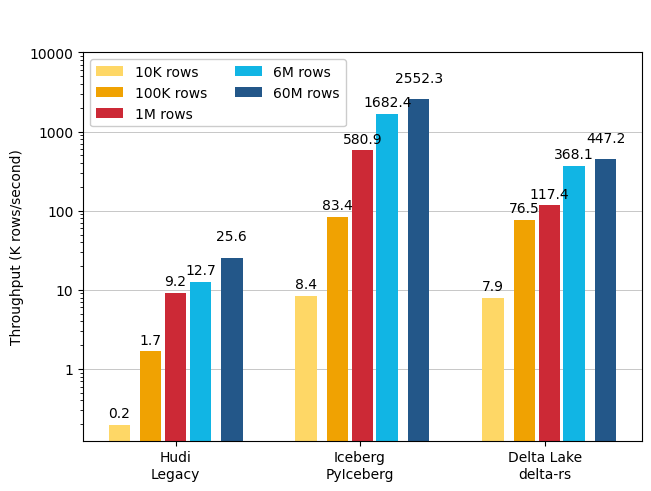
\includegraphics[width=\textwidth]{figures/7-appendix/results_diagrams/write/hudi_iceberg_delta/write_throughput_2_core.png}
        \caption[Histogram of the write experiment - Throughput - 2 CPU cores]{Histogram in log-scale of the write experiment results expressed as throughput. The experiment was performed with two \glstext{CPU} cores.}
        \label{fig:appx_res_write_throughput_2_cores_HID}
    \end{minipage}
\end{figure}

\begin{figure}
    \centering
    \begin{minipage}[b]{\textwidth}
        \centering
        \captionof{table}[Write experiment - Throughput - 4 CPU cores]{Write experiment results expressed as throughput. The experiment was performed with four \glstext{CPU} cores.}
        \label{tbl:appx_res_write_throughput_4_cores_HID}
        \begin{tabular}{c r S[table-format=7.5] S[table-format=7.5] S[table-format=7.5]} 
            \toprule
            \multirow{2}{*}{{Pipeline\Tstrut\Bstrut}} & \multirow{2}{*}{{\thead{Number\\ of rows}}} & {\multirow{2}{*}{{\thead{Throughput \\ (k rows/second)}}}} & \multicolumn{2}{c}{{\thead{Throughput (k rows/second) \\95\% Confidence Interval}}}\\
                                                      &                                             &                                                          & {low} & {high}\\
            \midrule
            \multirow{5}{4em}{Hudi\\Legacy}     &   10K   &     195.04029  &     192.61190  &     197.58999  \\
                                                &  100K   &    1680.27669  &    1662.85950  &    1699.08749  \\
                                                &    1M   &    9190.56612  &    9143.29267  &    9234.33987  \\
                                                &    6M   &   12449.19942  &   12424.92779  &   12474.40876  \\
                                                &   60M   &   25574.26227  &   25475.41012  &   25672.00975  \\
            \midrule
            \multirow{5}{4em}{Iceberg\\PyIceberg}  &   10K   &    8366.26993  &    8152.66704  &    8613.25608  \\
                                                   &  100K   &   79697.14780  &   77816.50315  &   82052.80544  \\
                                                   &    1M   &  612891.38485  &  597747.51880  &  630363.04983  \\
                                                   &    6M   & 1692583.43173  & 1680055.53315  & 1707255.44211  \\
                                                   &   60M   & 2499443.19781  & 2484091.83867  & 2510768.76960  \\
            \midrule
            \multirow{5}{4em}{Delta Lake\\delta-rs} &   10K   &    8218.02924  &    8109.88845  &    8316.83880  \\
                                                    &  100K   &   74820.47067  &   74050.66338  &   75578.59454  \\
                                                    &    1M   &  118784.11348  &  116237.35924  &  121271.60828  \\
                                                    &    6M   &  369835.13424  &  361760.40936  &  378999.43389  \\
                                                    &   60M   &  483631.53234  &  474129.46579  &  495203.23632  \\
            \bottomrule
        \end{tabular}
    \end{minipage}
    \begin{minipage}[b]{\textwidth}
        \centering
        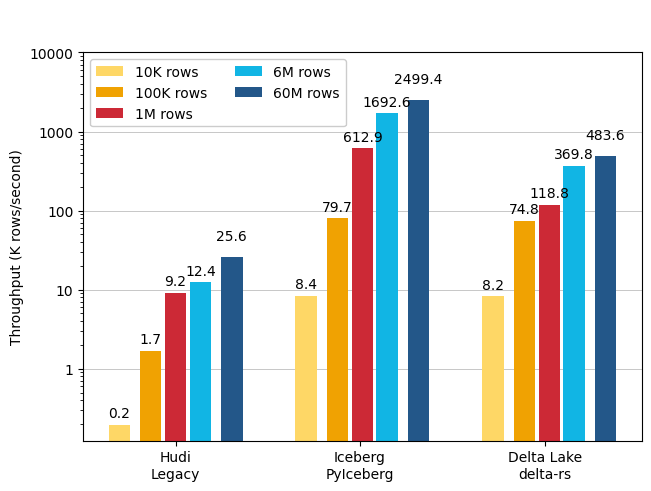
\includegraphics[width=\textwidth]{figures/7-appendix/results_diagrams/write/hudi_iceberg_delta/write_throughput_4_core.png}
        \caption[Histogram of the write experiment - Throughput - 4 CPU cores]{Histogram in log-scale of the write experiment results expressed as throughput. The experiment was performed with four \glstext{CPU} cores.}
        \label{fig:appx_res_write_throughput_4_cores_HID}
    \end{minipage}
\end{figure}

\begin{figure}
    \centering
    \begin{minipage}[b]{\textwidth}
        \centering
        \captionof{table}[Write experiment - Throughput - 8 CPU cores]{Write experiment results expressed as throughput. The experiment was performed with eight \glstext{CPU} cores.}
        \label{tbl:appx_res_write_throughput_8_cores_HID}
        \begin{tabular}{c r S[table-format=7.5] S[table-format=7.5] S[table-format=7.5]} 
            \toprule
            \multirow{2}{*}{{Pipeline\Tstrut\Bstrut}} & \multirow{2}{*}{{\thead{Number\\ of rows}}} & {\multirow{2}{*}{{\thead{Throughput \\ (k rows/second)}}}} & \multicolumn{2}{c}{{\thead{Throughput (k rows/second) \\95\% Confidence Interval}}}\\
                                                      &                                             &                                                          & {low} & {high}\\
            \midrule
            \multirow{5}{4em}{Hudi\\Legacy}     &   10K   &     195.21345  &     192.95222  &     197.67807  \\
                                                &  100K   &    1658.70267  &    1645.63630  &    1672.83862  \\
                                                &    1M   &    9142.28991  &    9103.09744  &    9181.79165  \\
                                                &    6M   &   12605.76130  &   12575.40944  &   12636.69010  \\
                                                &   60M   &   25808.58957  &   25739.09161  &   25871.43218  \\
            \midrule
            \multirow{5}{4em}{Iceberg\\PyIceberg}  &   10K   &    8208.72824  &    7747.34838  &    8627.10040  \\
                                                   &  100K   &   80090.88979  &   78352.19083  &   81977.33616  \\
                                                   &    1M   &  581707.82303  &  577533.98845  &  586819.41216  \\
                                                   &    6M   & 1698521.31195  & 1662196.40258  & 1727430.77830  \\
                                                   &   60M   & 2539884.06709  & 2531591.50316  & 2546589.00275  \\
            \midrule
            \multirow{5}{4em}{Delta Lake\\delta-rs} &   10K   &    7354.81049  &    6367.76735  &    8009.69774  \\
                                                    &  100K   &   77387.40941  &   76265.73288  &   79015.66143  \\
                                                    &    1M   &  120554.78447  &  118199.43031  &  122798.45207  \\
                                                    &    6M   &  381579.81360  &  370912.17014  &  393712.18390  \\
                                                    &   60M   &  492238.46299  &  483347.67878  &  502012.27941  \\
            \bottomrule
        \end{tabular}
    \end{minipage}
    \begin{minipage}[b]{\textwidth}
        \centering
        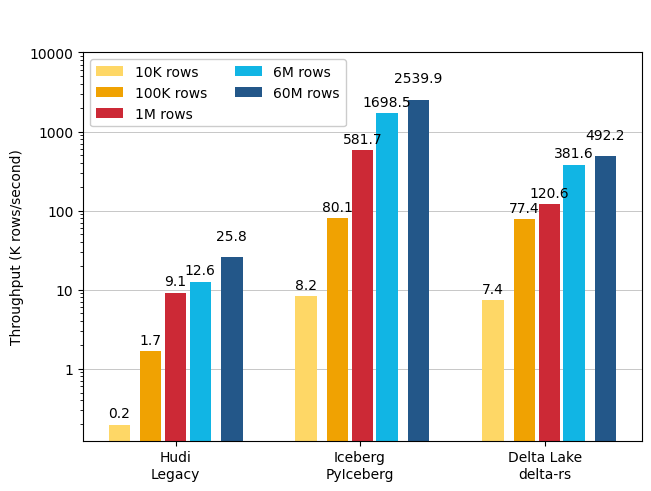
\includegraphics[width=\textwidth]{figures/7-appendix/results_diagrams/write/hudi_iceberg_delta/write_throughput_8_core.png}
        \caption[Histogram of the write experiment - Throughput - 8 CPU cores]{Histogram in log-scale of the write experiment results expressed as throughput. The experiment was performed with eight \glstext{CPU} cores.}
        \label{fig:appx_res_write_throughput_8_cores_HID}
    \end{minipage}
\end{figure}